
This section mainly reports our estimation and measurement result about the cpu operations and os service like system calls and context creation and switch.


\subsection{Overhead Measurement}
When performing measurement, we are using the following code to measure the overhead of a piece of code:

\lstinputlisting[language=C, firstline=4, lastline=15]{../include/proj_timing.h}

In the source code, we use RDTSC and RDTSCP to read out the timestamp counter register on the cpu. CPUID instruction serves as a barrier to ensure only cycles
runs between RDTSC and RDTSCP instructions will be counted. So when we want to measure the overhead of some functions (code pieces), we can just put START\_COUNT
before the target code pieces and STOP\_COUNT after, then we can easily get the cycles ticks during executing the code pieces we want to measure.


\subsubsection{Methodology}
When measuring the overhead of the measurement code we mentioned above, we use the following code snipes to perform the overhead measurement:

\lstinputlisting[language=C, firstline=21, lastline=22]{../CPU/time_ovh.c}

We just measure nothing between two count macros, so that this measurement will response the overhead of the execution of those two macros.

When performing the measurement, we will run the measurement code in a 10000 round loop, then we take the arithmetic mean of the cycles responsded as the final result.

% because this minimal
% cycles results can be an evidence that our cpu can finish running the target code within this minimal cycles ticks, and also, all other greater cycles ticks might imply that
% they are impacted by other infererence like hardware interruption. As a result, this minimal value is the value that most likely producing without any other infererence, so we take
% this minimal value as the measurement result.

\subsubsection{Estimation and Results}
\label{overhead_estimation}

The estimation and the measurement result will be list in the following table:

\begin{table}[ht]
  \centering
  \caption{\textbf{Measurement Overhead: Estimation and Experiment Results}}
  \begin{threeparttable}
  \begin{tabular}{ccccc}
  \hline
      \textbf{Hardware Overhead} & \textbf{Software Overhead } & \textbf{Total Overhead} & \textbf{Expr. Results} & \textbf{Standard} \\
      \textbf{Estimation}       &  \textbf{Estimation}         & \textbf{Estimation}  &   & \textbf{Deviation}  \\
  \hline
      6 (inst) or 44 (cycles) & 0 & 6 (instructions) & 102 & 3.8\\
  \hline
  \end{tabular}
  \end{threeparttable}
  \label{measurement_overhead_table}
\end{table}

When estimation, the first evidence for us to perform the estimation is the code we write and generate, following is the acutall assembly code after compilation:

\begin{lstlisting}
    4005f8:	0f a2                	cpuid
    4005fa:	0f 31                	rdtsc
    4005fc:	89 d7                	mov    %edx,%edi
    4005fe:	89 c6                	mov    %eax,%esi
    400600:	89 7d d0             	mov    %edi,-0x30(%rbp)
    400603:	89 75 d4             	mov    %esi,-0x2c(%rbp)
    400606:	0f 01 f9             	rdtscp
    400609:	89 d7                	mov    %edx,%edi
    40060b:	89 c6                	mov    %eax,%esi
    40060d:	0f a2                	cpuid
    40060f:	89 7d d8             	mov    %edi,-0x28(%rbp)
    400612:	89 75 dc             	mov    %esi,-0x24(%rbp)
\end{lstlisting}

We can found out: there are 4 instructions between RDTSC and RDTSCP instruction: two of them are inline assembly we write in code, and the rest two are compile-time generated code caused by
register saving, so the totally overhead for the measurement should be 4 instructions + 2 instructions (RDTSC and RDTSCP themselves).

The second issue for estimating the hardware overhead is that, how many cycles each instruction will take, or in other words, what is the cpu's CPI (cycles per instruction). We haven't found out
the most related information, so we performed the following estimation: for those 6 instructions, we assume that each cycle the cpu can commit one instruction, and the pipeline stages is around 20;
as those 6 instructions don't have any data dependencies that can not be solved by data forwarding, the pipeline will not stall, and for those 6 instructions, from first instruction enter the pipeline
to the last instruction commit, the cycles consumed should be:
    $$ 20 + 4 + 20 = 44 cycles $$

After the experiments, the result shows that we underestimated the overhead by around 50\%, but as we don't know much about the internal of the Intel CPU, so that this kind of mistakes is somewhat reasonable.

\subsection{Loop Overhead}
When performing estimation, it is reasonable that using repeated experiments to reduce the impact of variance, so before all other overhead measurement, we need to determine the overhead of the loop first.

\subsubsection{Methodology}

When measuring the loop overhead, we simply measures the cycles diff before and after a simple do nothing loop. In order to reduce the impact of variance, we also run this test 10000 times, and then take the arithmetic
means of 10000 samples. We also subtract the time measurement overhead (102 cycles as \textbf{Section \ref{overhead_estimation}}) from the loop overhead, so the final loop overhead should be:
    $$ average(cycles) - 102 $$

We also perform our measurement upon loops rounds from 0 to 50, in order to see the overhead of different loop scale.

\subsubsection{Estimation and results}

Our Estimation and the measurement results are shown in the \textbf{Figure \ref{loop_overhead_result}}:

\begin{figure}[ht]
    \centering
    \frame{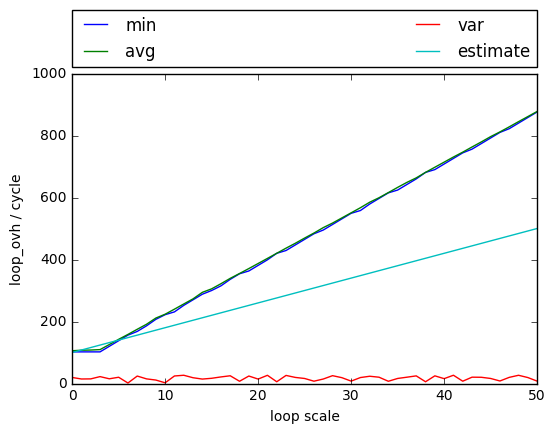
\includegraphics[width = .9\textwidth]{pictures/loop_ovh.png}}
    \caption{Loop Overhead: Estimation and Experiment Results }
    \label{loop_overhead_result}
\end{figure}

As shown in the graph, when estimating, we estimate the overhead increasing by 8 cycles when loop scale increase by 1. We made this estimate based on the instructions of the loop after compile:

\begin{lstlisting}
    4006a1:	c7 45 c4 00 00 00 00 	movl   $0x0,-0x3c(%rbp)
    4006a8:	eb 04                	jmp    4006ae <main+0xf8>
    4006aa:	83 45 c4 01          	addl   $0x1,-0x3c(%rbp)
    4006ae:	8b 45 c4             	mov    -0x3c(%rbp),%eax
    4006b1:	3b 45 c0             	cmp    -0x40(%rbp),%eax
    4006b4:	7c f4                	jl     4006aa <main+0xf4>
\end{lstlisting}

As shown in above, there will be 4 instructions for each round of the loop, as the \textbf{Section \ref{overhead_estimation}} shows that, each instruction will taken more than one cycle tick in average.
We finally made a assumption that each instructions will take up 2 cycles on average.

The result shows that we still underestimated the incremental ratio of the overhead, and in fact, each each loop round increase will increase the overhead by 18. The red line is the variance of our data, which shows our result is quite stable.

\subsection{Procedure Call}

\subsubsection{Methodology}

Since procedure call is very quick (our rough measurement shows it takes less than 10 cycles), we measure procedure calls in loops rather than individually to reduce the variance of the measurement's own overhead. The code is as following:

\begin{lstlisting}
for (i = 0; i < outerloop; i++) {
    START_COUNT();
    for (j=0; j < innerloop; j++){
        procedure_0();
    }
    STOP_COUNT();
}
\end{lstlisting}

When calculating the time consumed by procedure\_0, we first calculate the arithmetic mean of the duration cycles collected by START\_COUNT and STOP\_COUNT, then subtract the overhead of the time measurement and the innerloop from it, and finally divide the result by the innerloop times. We set outerloop and innerloop to be 10000 and 50 separately.

%When measuring the overhead of a procedure call, we just put our cycles counting code before and after the procedure call; also, we reduced the variance by using the arithmatic mean of the response overhead came from 10000 times measurements.

\subsubsection{Estimation and results}
We estimate the procedure call with no parameters will take 4 cycles and expect for two additional cycles for every one more parameter.

\textbf{Figure \ref{procedure_overhead_result}} shows our Estimation and the measurement results. The comparison indicates that procedure call is far more quicker than we expected and the overhead increases linearly when the parameter number increases. The variance line justifies that we have successfully eliminated most variance. There is a sudden jump on overhead between 2 and 3 parameters calls, and we speculate it is caused by the different alignments when the callees push 2 and 3
parameters to stack to save registers. 


\begin{figure}[h]
    \centering
    \frame{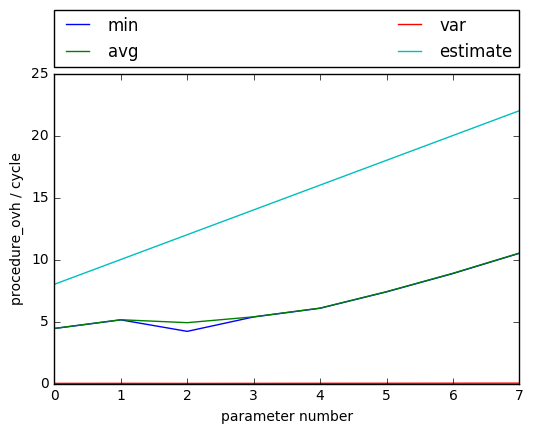
\includegraphics[width = .9\textwidth]{pictures/procedure.png}}
    \caption{Procedure Overhead: Estimation and Experiment Results }
    \label{procedure_overhead_result}
\end{figure}


\subsection{System Call}

\subsubsection{Methodology}

When measuring the system calls, basically we want to measure the cycle ticks between the begin and the return points of the system call. This means that we require the kernel return the control to the process immediately after the system call service routine finishes, so that what we can measure is some 'light weight' system call, like \textbf{getpid()} or \textbf{getcwd()}. However, \textbf{getpid()} will be cached by the kernel, so that only the first call of the getpid() can trap into
the kernel space, so that in the end, we choose \textbf{getcwd()} system call to be the system call we measured.

For specific implementation, the measurement process will first start counting cycles, then invoke \textbf{getcwd()} system call, finally stop counting. The cycles counted should be the overhead of the \textbf{getcwd()} system call.


\subsubsection{Estimation and results}

The estimation and the measurement results are shown in \textbf{Table \ref{measurement_syscall_table}}

\begin{table}[ht]
  \centering
  \caption{\textbf{System Call Overhead: Estimation and Experiment Results}}
  \begin{threeparttable}
  \begin{tabular}{ccccc}
  \hline
      \textbf{Hardware Overhead} & \textbf{Software Overhead } & \textbf{Total Overhead} & \textbf{Expr. Results} & \textbf{Standard}\\
      \textbf{Estimation}       &  \textbf{Estimation}         & \textbf{Estimation}  &     & \textbf{Deviation}\\
  \hline
  1000 inst & 0 & 1000 inst & 1250 & 31 \\
  \hline
  \end{tabular}
  \end{threeparttable}
  \label{measurement_syscall_table}
\end{table}

For estimation, system calls in a 64-bit system will first save a bunch of system call parameters into registers, then trap into the kernel by invoke \textbf{int} instruction or \textbf{syscall} instruction, then the kernel will serve the system call, and finally turn back to user mode with similar cost with trap into the memory. As there is a lot of assistance routine when traping into the system, then we believe 1000 cycle should be a reasonable estimation.

The results shows that our estimation is quite accurate.

For the questions about comparison between system call and procedure call, system call is definitely much heavy weight than procedure call, as a procedure call with 7 parameters only cost 11 cycles, but the system call will cost more than 1000 cycles. This is caused by a lot of checking and setting operations when traping into kernel mode and return to user mode.

\subsection{Process and Kernel Thread Creation}

\subsubsection{Methodology}
\label {creation_methodology}

When measuring Task, or process creation time, we need to ensure several things. The first one when the measurement process fork a child process after fork syscall, the os will schedule either the measurement process or the child of the measurement process to be executed. To ensure that, we run our measurement process with the round robin real time scheduler and set the process the highest priority. The cmd is as follows:

\begin{lstlisting}
    sudo chrt -rr 99 ./measurement
\end{lstlisting}

However, even we make our process the highest priority,  we are still not sure which process (parent, or child) will be executed first. So we need to ensure to handle both cases so that we can get the cycles between the point just before fork call and the point fork return.

In order to get the results we want, we implement the following measurement sequence:

\begin{enumerate}
    \item We initialize a pipe for child and parent process to communicate \label{task_creation_pipe}
    \item We start counting cycles before we call fork
    \item Both at the parent and the child process start point after fork return, we stop counting cycles
    \item Child process passing the end counting to the parent via the pipe we initialized at \textbf{\ref{task_creation_pipe}}
    \item We calculate both cycles spend for parent fork return and child fork return, then choose the smaller one (as the smaller one indicates that this process executes before the other one)
\end{enumerate}

For the kernel thread creation, we use a similar method. The measurement sequence is listed at following:
\begin{enumerate}
    \item We initialize a global variable for child process to store the end clock cycle count \label{thread_creation_gv}
    \item We start counting cycles before we call pthread\_create
    \item Both at the main and the peer thread start point after pthread\_create finished, we stop counting cycles
    \item peer thread passing the end counting to the main thread via the global variable we initialized at \textbf{\ref{thread_creation_gv}}
    \item We calculate both cycles spend for main thread pthread\_create return and pthread\_create start execution, then choose the smaller one (as the smaller one indicates that this thread executes before the other one)
\end{enumerate}

We repeat each measurement for 10000 times to get the accurate cycles.

\subsubsection{Estimation and results}

The estimation and the measurement result will be list in the \textbf{Table \ref{process_creation_time}}:

\begin{table}[ht]
  \centering
  \caption{\textbf{Process/Thread Creation Time: Estimation and Experiment Results}}
  \begin{threeparttable}
  \begin{tabular}{cccccc}
  \hline
      \textbf{Process or} & \textbf{HW Overhead} & \textbf{SW Overhead } & \textbf{Total Overhead} & \textbf{Expr. Results} & \textbf{Standard}\\
      \textbf{Kthread} & \textbf{Estimation}       &  \textbf{Estimation}         & \textbf{Estimation}  & (AVG)   & \textbf{Deviation} \\
  \hline
      \textbf{Process} & NA & NA & 20000 ($7.16 \mu s$) & 134507 & 3062 \\
      \textbf{Kernel Thread} & NA & NA & 10000 ($3.58 \mu s$) & 20635 & 1546 \\
  \hline
  \end{tabular}
  \end{threeparttable}
  \label{process_creation_time}
\end{table}

When we make estimation, it is hard for us to do the hard ware and software estimation, as there are a lot of issues hard to estimate. For example, for fork(), the kernel will create a new process control block for the new process, and then set
up a bunch of member's value inside the pcb; after that, it will at least initialize the child process's address space, by creating a bunch of page tables; all these operations might cost more then 20000 cycles. Compared with process creation,
thread creation is much more light weight, as thread doesn't need to construct a new address space. Finally we made a prediction that, process creation will cost 20000 cycles and thread will cost half of the process cost, 10000 cycles; or in other
word, $7.16 \mu s$ for process and $3.58 \mu s$ for thread.

Our experimental results show that the process creation and thread creation takes 134507 and 20635 cycles correspondingly, which means creating a process takes much longer time than we have estimated and creating a thread is much more lightweight. The standard deviations for our experiments are 3062 and 1546, which are relatively small to the average results.


\subsection{Process and Kernel Thread Context Switch}

\subsubsection{Methodology}

For the overhead measurement of the context switch, the basic idea to measure the overhead is to count the cycles spend on switch from one process (thread) to another process (thread). To make our measurement accurate, we need to ensure the same thing we indicates in
\textbf{section \ref{creation_methodology}}, that the measuring processes (threads) are the only two processes (threads) that to be scheduled. In the real system, this is impossible, but we can estimate this situation by increasing the priority of the process (threads).

For specific how to count the cycles of a context switch, we need to force a context switch to happen in one process (thread) the another (thread) process can stop the counting afterwards. To achieve this goal, we implement the following measure sequence by using blocking
reading pipe. To be more precisely, at parent process, we first start a pipe for communication, then fork new process; after that, parent process will first start counting cycles, then write to the communicating pipe, then call wait() to wait the child process; at the same time, child process will read from the pipe, then stop counting the cycles, and finally send the stop cycles back to the parent process via the pipe then exit; after that, parent will wake up and get the value and count the tick.

This method uses read and wait to synchronize. Either child or parent process executing first, the final result will be the period start from parent writing to the pipe, then context switch to the child, and finally the the child read from pipe.

The method for thread is similar, the differences are:

\begin{enumerate}
    \item We use pthread\_join() instead of wait()
    \item We use global variable, instead of pipe, to pass the final tick to the main thread;
\end{enumerate}


\subsubsection{Estimation and results}
\begin{table}[ht]
    \centering
    \caption{\textbf{Process/Thread Context Switch Time: Estimation and Experiment Results}}
    \begin{threeparttable}
        \begin{tabular}{cccccc}
        \hline
        \textbf{Process or} & \textbf{HW Overhead} & \textbf{SW Overhead } & \textbf{Total Overhead} & \textbf{Expr.        Results} & \textbf{Standard} \\
        \textbf{Kthread} & \textbf{Estimation}       &  \textbf{Estimation}         & \textbf{Estimation}  & (AVG)   & \textbf{Deviation}\\
        \hline
        \textbf{Process} & NA & NA & 20000 & 79097  &  650\\
        \textbf{Kernel Thread} & NA & NA & 10000 & 2562 & 538\\
        \hline
        \end{tabular}
    \end{threeparttable}
    \label{context_switch_time}
\end{table}

For the estimation of the overhead of a context switch, we are not pretty sure the precise overhead of the context switch, so we just make a guess that the overhead should be more then 10000 cycles for thread, and the overhead for the process should be at least twice as the thread's.

The final results shows that we under estimate the overhead of the process context switch, and it should be around 80000 cycles; but amazingly for the thread one, it only cost around 2500 cycles for context switch. We might perform some more measurement about that in the future.

For the question about difference between process context switch and kernel context switch, as the results show that, the overhead of thread context switch around 30 times less then process context switch. The main difference between thread and process context switch
is that, when thread context switching, kernel need neither to construct the virtual memory space to the thread switch to, nor to flush the tlb, which means that thread context switch is much less expensive than process context switch.
